\documentclass[DynamicalBook]{subfiles}
\begin{document}
%


\setcounter{chapter}{0}%Just finished 0.


%------------ Chapter ------------%
\chapter{Deterministic, Disrete-Time Systems}


Here's a basic fact of life: \emph{things change}. And how things change most
often depends on how they currently are. This is the basic idea underlying all the various notions of \emph{dynamical
  system} that we will see in this book.

\begin{informal}
  A \emph{dynamical system} consists of:
  \begin{itemize}
  \item a notion of how things are, called the \emph{state}, and
  \item a notion of how things will change given how they are, called the \emph{dynamics}.
  \end{itemize}
  The dynamics of a system might also depend on some free \emph{parameters}, and
  we will often only be interested in some particular \emph{variables} of the
  state. 
\end{informal}

In this chapter, we will see this idea in its
most distilled form: we will know exactly how things are, and what they will be
like next. That is, we'll be focusing on \emph{deterministic} dynamical systems,
whose time steps forward in \emph{discrete} increments.


A paradigmatic example of this sort of dynamical system is a clock.
\[
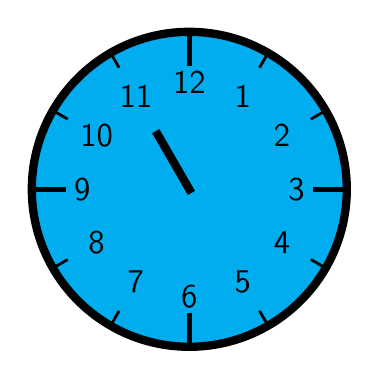
\begin{tikzpicture}[line cap=rect,line width=3pt]
\filldraw [fill=cyan] (0,0) circle [radius=2cm];
\foreach \angle [count=\xi] in {60,30,...,-270}
{
  \draw[line width=1pt] (\angle:1.8cm) -- (\angle:2cm);
  \node[font=\large] at (\angle:1.36cm) {\textsf{\xi}};
}
\foreach \angle in {0,90,180,270}
  \draw[line width=2pt] (\angle:1.6cm) -- (\angle:2cm);
\draw (0,0) -- (120:0.8cm);
\end{tikzpicture}
\]

Suppose that our clock has just an hour hand for now. Then we may collect all
the way things can be for the clock into a set of hours:
$$\Set{Hours} := \{1, 2, 3, 4, 5, 6, 7, 8, 9, 10, 11, 12\}.$$

The set $\Set{Hours}$ is the set of \emph{states} of our clock system. If we know what hour it is, we also know what hour is coming next. So, this system has the following dynamics:
%
% :CUSTOM-ID: problem-with-drawing-mapsto-nicely
%
\begin{align*}
  \fun{tick} : \Set{Hours} &\to \Set{Hours} \\
                t &\mapsto \begin{cases} t + 1 &\mbox{if $t < 12$}\\ 1 &\mbox{if $t = 12$}  \end{cases}
\end{align*}

Here's a sample of the dynamics of the clock. Say we started at 3 o'clock:
$$3 \xmapsto{\fun{tick}} 4 \xmapsto{\fun{tick}} 5 \xmapsto{\fun{tick}} 6
\xmapsto{\fun{tick}} \cdots$$

Not the most dynamic of systems, but we have to start somewhere. If we want to
refer to the whole system at once, we can box it up and write it like this:

\begin{equation}\label{eqn.clock_system_box}\tag{Clock System}
\begin{tikzpicture}[oriented WD, bbx = 1cm, bby =.5cm, bb min width=1cm, bb port length=4pt, bb port sep=1]
	\node[bb={0}{1}] (X) {$\Sys{Clock}$};
	\draw[label] 
		node [right=2pt of X_out1] {$\Set{Hours}$}
		;
\end{tikzpicture}
\end{equation}

We imagine that the clock is going about its business inside the clock, and
that is shows the hour it is currently displaying on the outgoing wire.

One issue with our clock is that it doesn't tell us whether it is morning or
evening. Being morning or evening is its own way that things might be, and we
can see it as its own dynamical system. We might imagine a little addition to
our clock that reads $\const{a.m.}$ or $\const{p.m.}$:
\begin{equation}\label{eqn.whole_clock}
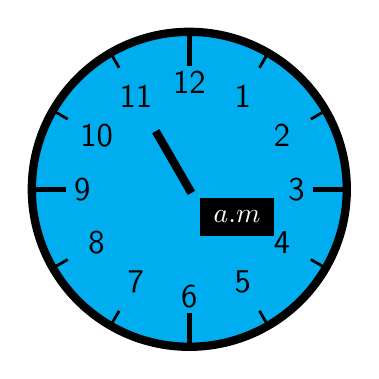
\begin{tikzpicture}[line cap=rect,line width=3pt]
\filldraw [fill=cyan] (0,0) circle [radius=2cm];
\foreach \angle [count=\xi] in {60,30,...,-270}
{
  \draw[line width=1pt] (\angle:1.8cm) -- (\angle:2cm);
  \node[font=\large] at (\angle:1.36cm) {\textsf{\xi}};
}
\foreach \angle in {0,90,180,270}
  \draw[line width=2pt] (\angle:1.6cm) -- (\angle:2cm);
\draw (0,0) -- (120:0.8cm);
\node[draw, fill] at (330:.7cm) {$\color{white}\const{a.m}$};
\end{tikzpicture}
\end{equation}

We can see this little addition as a system in its own right; it is the system
of $\const{a.m.}/\const{p.m.}$. The states of this system are
$$\Set{Meridien} = \{\const{a.m.}, \const{p.m.}\}.$$
But this time, knowing how they are going to change also requires us to know the
hour:
\begin{align*}
  \fun{next} : \Set{Meridien} \times \Set{Hours} &\to \Set{Meridien} \\
               (\const{a.m}, t) &\mapsto \begin{cases} \const{p.m.} &\mbox{if $t = 11$}\\ \const{a.m} &\mbox{otherwise}  \end{cases} \\
               (\const{p.m}, t) &\mapsto \begin{cases} \const{a.m.} &\mbox{if $t = 11$}\\ \const{p.m} &\mbox{otherwise}  \end{cases}
\end{align*}
If it is $\const{a.m.}$ and the clock reads 8, then it will still be
$\const{a.m.}$; but if it is $\const{a.m.}$ and the clock reads 11, then it will
switch on the next hour to $\const{p.m.}$.

The thing to note about the dynamics of the $\const{a.m.}/\const{p.m.}$ system
is that they depend on what hour it is. The hour is a \emph{parameter} for the
dynamics of this system. We can draw this system as a box like this:
\begin{equation}\label{eqn.am_pm_system_box}
\begin{tikzpicture}[oriented WD, bbx = 1cm, bby =.5cm, bb min width=1cm, bb port length=4pt, bb port sep=1]
	\node[bb={1}{1}] (X) {$\Sys{a.m./p.m.}$};
	\draw[label] 
		node [left=2pt of X_in1] {$\Set{Hours}$}
		node [right=2pt of X_out1] {$\Set{Meridien}$}
		;
\end{tikzpicture}
\end{equation}
We have the $\Set{Meridien}$ wire coming out, which carries the information of
whether it is $\const{a.m.}$ or $\const{p.m.}$, just like the clock. But we also
have a wire coming in, which carries the hour that we need as a parameter for
our dynamics.


We can now express our whole clock (\ref{eqn.whole_clock}) by wiring together
our bare clock and the $\const{a.m.}/\const{p.m.}$ system:

\begin{equation}\label{eqn.clock_system_box}
\begin{tikzpicture}[oriented WD, bbx = .3cm, bby =.3cm, bb min width=.5cm, bb port length=2pt, bb port sep=1]
	\node[bb={1}{1}] (X1) {$\Sys{a.m./p.m.}$};
  	\node[bb={0}{1}, below=of X1] (X2) {$\Sys{Clock}$};
	\node[bb={0}{2}, fit={($(X1.north west)+(-2,1)$) ($(X1.north east)+(2,1)$) ($(X2.south)+(0,-3)$)}] (Y) {};
  \node[above=0pt of Y.south] (Label) {$\Sys{ClockWithDisplay}$};
	\draw (X1_out1) to (Y_out1);
  \draw (X2_out1) to[out=0, in=0] (2,-1.5);
  \draw (1.9, -1.5) to (-2.9, -1.5);
  \draw (-3, -1.5) to[out=180, in=180] (X1_in1);
  \draw (X2_out1) to (Y_out2);
	\draw[label] 
		node [right=2pt of Y_out1] {$\Set{Meridien}$}
		node [right=2pt of Y_out2] {$\Set{Hours}$}
		;
\end{tikzpicture}
\end{equation}

This system has states
$$\Set{HoursWithDisplay} := \Set{Hours} \times \Set{Meridien}$$
consisting of a pair $(11, \const{a.m.})$ of an hour and a meridien reading.
They update in a combined way, by using the hour shown on the clock face as the
parameter we need for the $\const{a.m.}/\const{p.m.}$ system. In full, the
dynamics looks like this:
\begin{align*}
  \fun{tick'} :\Set{HoursWithDisplay} &\to \Set{HoursWithDisplay} \\
  (t, m) &\mapsto (\fun{tick}(t), \fun{next}(t, m))
\end{align*}

\begin{exercise}
  Expand the definition of the combined system out in full, and check that it
  really does behave like the clock with $\const{a.m.}/\const{p.m.}$ display should.
\end{exercise}

Now that we have a working clock, we can use it for systems that need to know
the time. For example, consider a diner that opens at $7 \const{a.m.}$ and
closes at $10 \const{p.m.}$. The states of this diner are
$$\Set{DinerState} = \{\const{open}, \const{closed}\}.$$
The diner's dynamics are then
\begin{align*}
  \fun{dinerDynamics} : \Set{DinerState} \times \Set{HoursWithDisplay} &\to \Set{DinerState} \\
  (\const{open}, (10, \const{p.m.})) &\mapsto \const{closed} \\
  (\const{closed}, (7, \const{a.m.})) &\mapsto \const{open} \\
  (s, (t, m)) &\mapsto s \quad\mbox{otherwise.} 
\end{align*}

Again, we can represent the diner by this box:
\begin{equation}\label{eqn.diner_system_box}\tag{box1}
\begin{tikzpicture}[oriented WD, bbx = 1cm, bby =.5cm, bb min width=1cm, bb port length=4pt, bb port sep=1]
	\node[bb={2}{1}] (X) {$\Sys{Diner}$};
	\draw[label] 
		node [left=2pt of X_in1] {$\Set{Meridien}$}
		node [left=2pt of X_in2] {$\Set{Hours}$}
		node [right=2pt of X_out1] {$\Set{DinerState}$}
		;
\end{tikzpicture}
\end{equation}
This time, we have two wires coming in, corresponding to the two parameters we
need for the diner system: the hour and the
meridien. 

Assuming that the diner has a clock on its wall which it uses to decide whether
to open or close, the full diner system would be given by wiring the clock with display into
those input wires:
\begin{equation}\label{eqn.diner_system_box}\tag{box1}
\begin{tikzpicture}[oriented WD, bbx = 1cm, bby =.5cm, bb min width=1cm, bb port length=4pt, bb port sep=1]
	\node[bb={1}{1}] (X) {$M$};
	\draw[label] 
		node [left=2pt of X_in1] {$A$}
		node [right=2pt of X_out1] {$B$}
		;
\end{tikzpicture}
\end{equation}
If we want to, we can peak into the clock with display and see that it is itself
made out of a clock wired to a display:
\begin{equation}\label{eqn.diner_system_box}\tag{box1}
\begin{tikzpicture}[oriented WD, bbx = 1cm, bby =.5cm, bb min width=1cm, bb port length=4pt, bb port sep=1]
	\node[bb={1}{1}] (X) {$M$};
	\draw[label] 
		node [left=2pt of X_in1] {$A$}
		node [right=2pt of X_out1] {$B$}
		;
\end{tikzpicture}
\end{equation}

We call this way of putting together dynamical systems to make more complex
systems \emph{composition}.
\begin{informal}
  \emph{Composition} is the process by which some things are brought together to
  form bigger things.

  Functions can be composed by $g \circ f(x) = g(f(x))$, and dynamical systems
  can be composed by plugging in the variables of the states of some into the
  parameters of others.
\end{informal}

This book is all about composing dynamical systems. Because of this, we will use
the abstract language of composition: \emph{category theory}.
\begin{informal}
\emph{Category theory} is the abstract study of composition.
\end{informal}


That's a lot of informal definitions, we are ready for something precise:
\begin{definition}
  A \emph{deterministic system} $\lens{u}{r} : \lens{S}{S} \leftrightarrows \lens{I}{O}$ consists of:
  \begin{itemize}
    \item A set $S$ of \emph{states}.
    \item A set $O$ of \emph{values for exposed variables}, or \emph{outputs}
      for short.
    \item A set $I$ of \emph{parameter values}, or \emph{inputs} for short.
    \item A function $r : S \to O$, the \emph{exposed variable of state} or
      \emph{readout} function which takes a state to the output it yields. 
    \item A function $u : S \times I \to S$, the \emph{dynamics} of
      \emph{update} function which takes a state and a parameter and gives the
      next state.
  \end{itemize}
  We refer to the pair $\lens{I}{O}$ of exposed variable and parameter values as
  the \emph{interface} of the system.
\end{definition}

\section{Wiring Together Systems with Lenses}

\end{document}
